\section[Komplexitätstheorie]{Komplexitätstheorie}
% \subsection{Komplexitätsklassen und \ac{P}/\ac{NP}}

In der Informatik II Vorlesung betrachteten Sie Algorithmen und lernten Sie den ``Worst Case'' Ressourcenverbrauch von diesen zu bestimmen.
In diesem Kapitel der Vorlesung werden wir nun Problemstellungen betrachten und versuchen den Worst Case Ressourcenverbrauch des bestmöglichen Algorithmus zu bestimmen.

Wir betrachten zwei Arten von Ressourcen; Laufzeit und benötigter Speicherplatz.
Für \acp{TM} formalisieren wir diese wie folgt.

\begin{Def}
Sei $f:\N\rightarrow\N$ eine Funktion und $\M$ eine \ac{TM} mit Eingabealphabet $\Sigma$.
\begin{itemize}
 \item $\M$ hat \emph{Zeitkomplexität} $f(n)$, falls $\forall w\in\Sigma^*$ mit Länge $n$ gilt: $\M$ hält auf Eingabe $w$ für jede Berechnung in höchstens $f(n)$ Schritten.
 \item $\M$ hat \emph{Platzkomplexität} $f(n)$, falls $\forall w\in\Sigma^*$ mit Länge $n$ gilt: Wenn $\M$ auf $w$ angesetzt wird, benutzt jede Berechnung höchstens $f(n)$ Bandzellen.
 \qedhere
\end{itemize}
\end{Def}


Um Problemstellungen besser miteinander vergleichen zu können beschreiben wir diese als Wortproblem für Sprachen.
Die Frage ob eine aussagenlogische Formel $F$ erfüllbar ist formulieren wir z.B. als:
``Liegt $F$ in der Menge der erfüllbaren aussagenlogischen Formeln? ``
Wir klassifizieren nun Sprachen entsprechend des Ressourcenverbrauchs von \acp{TM} die diese akzeptieren.


\begin{Def}[name={[$\NTIME$ Klasse]}]
	Sei $f:\N\->\N$ eine Funktion.
	\begin{align*}
	\DTIME(f(n)) := \{L \subseteq\Sigma^*\mid & \text{ Es gibt det. Mehrband-\ac{TM} $\M$,}\\
	                & \text{sodass $L(\M)=L$ und $\M$ Zeitkomplexität $f(n)$ hat.} \}\\
%     \end{align*}
%     \begin{align*}
    \NTIME(f(n)) := \{L \subseteq\Sigma^*\mid & \text{ Es gibt nichtdet. Mehrband-\ac{TM} $\M$,}\\
                    & \text{sodass $L(\M)=L$ und $\M$ Zeitkomplexität $f(n)$ hat.} \}\\           
%     \end{align*}
% 	\begin{align*}
	\DSPACE(f(n)) := \{L \subseteq\Sigma^*\mid & \text{ Es gibt det. Mehrband-\ac{TM} $\M$,}\\
	                & \text{sodass $L(\M)=L$ und $\M$ Platzkomplexität $f(n)$ hat.} \}\\
%     \end{align*}
%     \begin{align*}
    \NSPACE(f(n)) := \{L \subseteq\Sigma^*\mid & \text{ Es gibt nichtdet. Mehrband-\ac{TM} $\M$,}\\
                    & \text{sodass $L(\M)=L$ und $\M$ Platzkomplexität $f(n)$ hat.} \}\qedhere
    \end{align*}	

% 	Die Klasse $\NTIME(f(n))$ besteht aus allen Sprachen, die von einer (Mehrkanal-)\ac{TM} $M$ in $T_M(w)\leq f(|w|)$ akzeptiert werden.\\
% 	Dabei $T_M(w) =
% 	\begin{cases}
% 		\mathrlap{\text{Anzahl der Schritte einer kürzesten akzeptierenden Berechnung von $M$ auf }w}\\
% 		1 & \text{falls }\nexists
% 	\end{cases}$\\
\end{Def}


\begin{figure}[htb]
	\begin{center}
		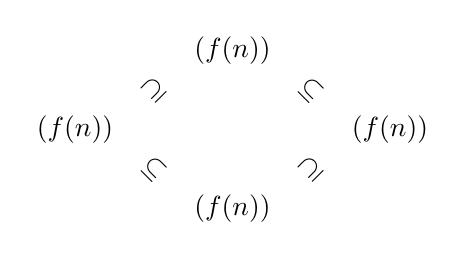
\begin{tikzpicture}
			\node (dtime) at (0,1) {$\DTIME(f(n))$};
			\node (ntime) at (2,0) {$\NTIME(f(n))$};
			\node (dspace) at (-2,0) {$\DSPACE(f(n))$};
			\node (nspace) at (0,-1) {$\NSPACE(f(n))$};
			\path (dtime) to node[rotate=-45] {$\subseteq$} (ntime);
			\path (dtime) to node[rotate=45] {$\supseteq$} (dspace);
			\path (ntime) to node[rotate=45] {$\supseteq$} (nspace);
			\path (dspace) to node[rotate=-45] {$\subseteq$} (nspace);
		\end{tikzpicture}
	\end{center}
	\caption{Inklusionsrelationen zwischen Komplexitätsklassen}
\end{figure}


Wir wollen im Folgenden Probleme als Sprachen darstellen und beginnen zunächst mit dem Erfüllbarkeitsproblem der Aussagenlogik.

\goodbreak

\textbf{Aussagenlogische Formeln als Sprachen}

Wir gehen davon aus, dass die Leser des Skripts mit \ac{AL}\footnote{%
Eine Einführung in Aussagenlogik finden Sie im Skript zur Vorlesung \emph{Logik für Studierende der Informatik} aus dem WS 2017/18.
Wir werden in dieser Vorlesung eine sehr ähnliche Notation verwenden.
\url{http://home.mathematik.uni-freiburg.de/junker/ws17/logik-info.html}
}
vertraut sind, stellen die von uns verwendete Syntax vor und bitten den Leser, sich die entsprechende Semantik zu erschließen.

Im Folgenden möchten wir Mengen von \ac{AL}-Formeln als Sprachen beschreiben.
Dafür müssen wir zunächst ein geeignetes Alphabet wählen.
Dabei nehmen wir "`0"' und "`1"' für die Konstanten,
"`$\neg$"', "`$\land$"' und "`$\lor$"' für die Junktoren
und runde Klammern "`$($"' und "`$)$"'.
Bei der Darstellung der Aussagenvariablen stehen wir nun vor der folgenden Herausforderung:
Es gibt unendliche viele Aussagenvariablen $A_0,A_1,A_2,A_3,\ldots$, aber unser Alphabet kann nur endlich viele Zeichen haben.
Unsere Lösung dafür ist sehr ähnlich wie die, die wir auch auf Papier verwenden.
Wir stellen eine Aussagenvariable durch ein "`$A$"' dar, das von einer Ziffernfolge gefolgt wird.
Die Aussagenvariable $A_{1337}$ wir so durch das Wort $A1337$ der Länge 5 repräsentiert.
Wir müssen unser Alphabet also noch um "`$A$"', "`$2$"', $\ldots$ "`$9$"' ergänzen und erhalten
$$\Sigma_\mathsf{AL}=\{0,1,2,3,4,5,6,7,8,9,A,\neg,\land,\lor,(,)\}.$$

\begin{Def}\label{def:gal}
Die Menge der \ac{AL}-Formeln ist die Sprache der kontextfreien Grammatik
  $\mathcal{G}_\mathsf{AL} = (\Sigma_\mathsf{AL}, N, P, S)$ mit
	\begin{align*}
		N &= \{S,Z\}\\
		P &= \begin{aligned}[t]
      \{ S \to\ & 0\mid 1\mid AZ\mid \neg S\mid (S\land S)\mid (S\lor S)\\
        Z \to\ & 0Z\mid 1Z\mid 2Z\mid 3Z\mid 4Z\mid 5Z\mid 6Z\mid 7Z\mid 8Z\mid 9Z \mid \\
        &0 \mid 1 \mid 2 \mid 3 \mid 4 \mid 5 \mid 6 \mid 7 \mid 8 \mid 9\}.
        \end{aligned}
      \qedherefixaligned
	\end{align*}
\end{Def}

Wir nehmen nun unsere Definition von Formeln, um ein bekanntes Problem mit Hilfe einer Sprache zu beschreiben.
\begin{Def}
Wir nennen die Menge der erfüllbaren \ac{AL}-Formeln \acsu{SAT}.
\[ \ac{SAT}=\{F\mid F\in L(\mathcal{G}_\mathsf{AL}) \text{ und $F$ erfüllbar}\}\qedhere \]
\end{Def}


Wir können nun also die Frage, ob die Formel $F$ erfüllbar ist, als Wortproblem "`$F\in\ac{SAT}?$"' darstellen.
Wir wollen im Folgenden eine \ac{TM} konstruieren, die \ac{SAT} entscheidet, betrachten aber als Vorstufe hierfür zunächst eine einfachere Sprache.


Wir definieren uns $\mathcal{G}_\mathsf{AL0}$ als die obige Grammatik, in der die Regel $S\to AZ$ fehlt.
Offensichtlich enthält $L(\mathcal{G}_\mathsf{AL0})$ genau die \ac{AL}-Formeln, die keine Aussagenvariablen enthalten.

Weiter definieren wir 
$$\text{SAT}_0=\{F\mid F\in L(\mathcal{G}_\mathsf{AL0}) \text{ und $F$ erfüllbar}\}$$
und konstruieren eine \ac{DTM}, die $\text{SAT}_0$ entscheidet.

\begin{Bsp}\label{bsp:DtmSat0}
Sei $\M_{\text{SAT}_0}$ eine \ac{DTM}, deren Verhalten wir wie folgt informell beschreiben.
\begin{itemize}
 \item Grundlegende Idee: Laufe von links nach rechts über die Eingabe und ersetze alle Operationen auf Konstantensymbolen direkt durch das Ergebnis (z.B. $1\land 0\rightsquigarrow 0$).
 Wiederhole dies, bis $0$ oder $1$ auf dem Band steht.
 \item Problem: Das Resultat dieser Operationen hat weniger Zeichen als die Eingabe.
 \item Lösung: Erweitere das Bandalphabet um ein Zeichen $\blacksquare$, um entstandene Leerstellen zu markieren (z.B. $1\land 0\rightsquigarrow 0\blacksquare\blacksquare$). Alternative: Verschiebe den Bandinhalt entsprechend.
 \qedhere
\end{itemize}
\end{Bsp}

\begin{description}
\item[Frage:] Was ist die bestmögliche Zeitkomplexität, die wir für $\M_{\text{SAT}_0}$ geben können?

\item[Antwort:] Wir müssen im schlimmsten Fall für jeden Operator einmal über die Eingabe laufen.
Die Zeitkomplexität ist also "`garantiert nicht viel schlimmer als $n^2$"', wobei $n$ die Größe der Eingabe ist.
Wir können die Zeitkomplexität aber nicht exakt angeben, da die Beschreibung von $\M_{\text{SAT}_0}$ zu unpräzise ist.
(Läuft der Kopf gelegentlich links und rechts über die Eingabe hinaus um das Wortende zu bestimmen?
Läuft der Kopf beim Ersetzen zurück?)
\end{description}

Ein Formalismus zum Beschreiben von Aussagen wie "`garantiert nicht viel schlimmer als \dots"'
ist das (große) $\mathcal{O}$-Symbol der Bachmann–Landau-Notation.
Wir gehen davon aus, dass die Leser des Skripts mit diesem Formalismus vertraut sind, wollen die Definition von (groß) $\mathcal{O}$ hier aber nochmal wiederholen.

\begin{Def} Sei $g:\N\rightarrow\N$.
\[ \mathcal{O}(g(n)) = \{f:\N\rightarrow\N \mid \exists n_0, k\in\N:\, \forall n\geq n_0: f(n)\leq k\cdot g(n)\} \qedhere \]
\end{Def}
Die Klasse $\mathcal{O}(g(n))$ enthält also genau die Funktionen, die für "`große Argumente"' durch ein Vielfaches von $g(n)$ beschränkt sind.

Über die Schwierigkeit von $\text{SAT}_0$ können wir nun also sagen:
Es gibt ein $f(n)\in\mathcal{O}(n^2)$, sodass $\text{SAT}_0\in\DTIME(f(n))$.

\begin{Bsp}\label{bsp:NtmSat}
Sei $\M_\text{SAT}$ eine \ac{NTM}, deren Verhalten wir wie folgt informell beschreiben.
\begin{itemize}
 \item Phase 1: Laufe über die Eingabe, sammle alle Aussagenvariablen $A_{k_1},\ldots,A_{k_n}$, rate (wähle nichtdeterministisch) für jede davon eine Belegung $b_{k_i}$ und schreibe
 $$A_{k_1}=b_{k_1},\quad\ldots,\quad A_{k_n}=b_{k_n}$$
 auf ein zweites Band.
 Dabei soll jede Variable höchstens einmal geschrieben werden, auch wenn sie mehrfach in der Eingabe vorkommt.
  
 Zeitkomplexität: 
 Ein Vergleich zweier Aussagenvariablen ist in $\mathcal{O}(n)$ möglich,
 pro Variablen müssen höchstens $\mathcal{O}(n)$ Vergleiche gemacht werden und
 in der Eingabe sind höchstens $\mathcal{O}(n)$ Variablen enthalten.
 Die Zeitkomplexität von Phase 1 kann also durch $\mathcal{O}(n^3)$ beschränkt werden.
 
 \item Phase 2: Laufe über die Eingabe und ersetze alle Aussagenvariablen durch die geratene Belegung.
 
 Zeitkomplexität: Durch $\mathcal{O}(n^3)$ beschränkt, nahezu gleiche Argumentation wie oben.
 
 \item Phase 3: Wende die in \autoref{bsp:NtmSat} beschriebene \ac{DTM} $\M_{\text{SAT}_0}$ auf den Bandinhalt an.
 
 Zeitkomplexität: Durch $\mathcal{O}(n)^2$ beschränkt.
\end{itemize}
Die Zeitkomplexität von $\M_\text{SAT}$ ist also durch $\mathcal{O}(n^3)$ beschränkt.
\end{Bsp}


\datenote{01.02.2019}
Über die Schwierigkeit von \ac{SAT} können wir somit sagen:
Es gibt ein $f(n)\in\mathcal{O}(n^3)$, sodass $\ac{SAT}\in\NTIME(f(n))$.



\begin{description}
 \item[Frage:] Angenommen, wir möchten ein schnelles Entscheidungsverfahren für \ac{SAT} implementieren.
Hilft uns dann die Konstruktionsidee von $\M_\text{SAT}$?
 \item[Antwort:] Eher nein. 
Die Konstruktion basiert darauf, dass wir nichtdeterministisch eine Belegung "`raten"'.
Es ist unklar, wie wir diesen Nichtdeterminismus auf einem (deterministischen) Computer effizient implementieren können.
Eine Möglichkeit wäre analog zum Beweis von \autoref{satz:Ntm2Dtm} alle nichtdeterministischen Wahlmöglichkeiten zu simulieren.
Da wir $\M_\text{SAT}$ aber pro Aussagenvariable nichtdeterministisch zwischen $0$ und $1$ wählen können, wäre das Verfolgen aller Wahlmöglichkeiten nur mit exponentiellem Aufwand möglich.
\end{description}

\begin{description}
 \item[Frage:] Gibt es ein "`schnelles"' Entscheidungsverfahren für \ac{SAT} oder ist das Problem so schwierig, dass es kein solches Verfahren geben kann?
 \item[Antwort:] Die Informatik kann bisher (Stand Januar 2019) auf beide Frageteile keine Antwort liefern. 
 Wir stellen aber im Folgenden einen Formalismus vor, mit dem sich diese Frage präziser formulieren lässt und wir für verwandte Fragen hilfreichere Antworten liefern können.
\end{description}


Um Missverständnisse in Terminologie und Notation zu vermeiden, wiederholen wir hier nochmal die aus der Schule bekannte Definition eines Polynoms.

\begin{Def}[name={[Polynom]}]
	Ein Polynom ist eine Funktion $p:\N\->\N$ mit $\exists k\in \N\ a_0,\dots,a_k\in\N$ und \mbox{$p(n)=\sum_i^k a_in^k$}
\end{Def}
\begin{Bemerkung}
 Die Funktion $f(n)=2^n$ ist kein Polynom, da $n$ hier ein Exponent ist.
\end{Bemerkung}

\begin{Def}
 \begin{align*}
  \acsu{P} &= \bigcup_{p\text{ Polynom}} \DTIME(p(n)) \\
  \acsu{NP} &= \bigcup_{p\text{ Polynom}} \NTIME(p(n))
  \qedhere
 \end{align*}
\end{Def}

\begin{Bemerkung}
 Die Laufzeitanalysen der \ac{TM}s aus \autoref{bsp:DtmSat0} und \autoref{bsp:NtmSat} zeigen, dass $\text{SAT}_0\in P$ und $\ac{SAT}\in \ac{NP}$.
\end{Bemerkung}


% \begin{Def}[name={[NP-Klasse]}]
% 	Die Klasse \ac{NP} besteht aus allen Sprachen, die von \ac{NTM} in polynomieller Zeit akzeptiert werden können.
% 	\[ \ac{NP} = \cup_{p\text{ Polynom}} \NTIME(p(n)) \]
% \end{Def}
% Analog für deterministische TM:
% \begin{Def}[name={[$\DTIME$ Klasse]}]
% 	Sei $f:\N\->\N$ Funktion\\
% 	$\DTIME(f(n)) =$ Klasse der Sprachen, die von \ac{DTM} in $T_M(w)\leq f(|w|)$ Schritten akzeptiert wird.
% 	\[ \ac{P} = \cup_{p\text{ Polynom}} DTIME(P(n)) \qedhere \]
% \end{Def}
Offensichtlich gilt $P\subseteq \ac{NP}$, da die \ac{DTM} ein Spezialfall der \ac{NTM} ist.
Die Frage, ob $P=\ac{NP}$ oder $P\neq \ac{NP}$ gilt, wurde bereits 1971 von Stephen Cook gestellt und ist das vermutlich bekannteste ungelöste Problem der Informatik.

Das "`\ac{P} vs. \ac{NP}"'-Problem ist auch deshalb interessant, weil es eine Vielzahl praxisrelevanter Problemstellungen gibt (Travelling Salesman, Erfüllbarkeit der Aussagenlogik, \dots),
die in \ac{NP} liegen, aber für die bisher nur (deterministische) Algorithmen mit mindestens exponentieller Laufzeit gefunden wurden.

Angenommen, wir wollen in unserem Unternehmen ein neues Problem lösen
(z.B. automatisches Verteilen von miteinander kommunizierenden Benutzern auf verschiedene Server, sodass die Netzwerklast am geringsten ist).
Angenommen, wir wissen bereits,
\begin{itemize}
 \item dass wir das Problem mit einer \ac{NTM} in polynomieller Zeit lösen könnten,
 \item dass für unsere Eingabegrößen eine polynomielle Laufzeit noch akzeptabel, aber eine exponentielle Laufzeit nicht mehr akzeptabel wäre und
 \item dass es einen approximativen Algorithmus gibt, der polynomielle Laufzeit hat, aber nicht immer optimale Resultate liefert.
\end{itemize}
Wie gehen wir nun weiter vor? Suchen wir nach einem (exakten) Algorithmus mit polynomieller Laufzeit oder geben wir auf und implementieren den approximativen Algorithmus?

Wir stellen im Folgenden einen Formalismus vor, mit dem wir
% unter bestimmten umständen 
Aussagen der folgenden Form machen können:
"`Ich weiß zwar nicht, ob meine neues Problem in \ac{P} liegt oder nicht.
Ich weiß aber, dass mein Problem so schwierig ist, dass das Finden eines polynomiellen Algorithmus \ac{P} = \ac{NP} implizieren würde."'

\begin{Def}[Polynomielle Reduktion]\label{def:PolyReduktion}
	Seien $U, V \subseteq \Sigma^*$ Sprachen.
  \emph{$U$ ist auf $V$ polynomiell reduzierbar}, falls eine totale, berechenbare Funktion
  $f:\Sigma^* \to \Sigma^*$ existiert, sodass
  \begin{itemize}
   \item $\forall w \in \Sigma^*:w \in U \iff f(w) \in V$
   \item $f$ wird von einer \ac{DTM} berechnet, deren Zeitkomplexität ein Polynom ist.
  \end{itemize}
  gilt.
  Wir nennen $f$ \emph{Reduktionsfunktion}
  außerdem nennen wir die zugehörige binäre Relation auf Sprachen die \emph{Reduktionsrelation}
  und schreiben $U \preceq_p V$ wenn $U$ auf $V$ polynomiell reduzierbar ist.
\end{Def}


% \datenote{02.02.2018}
Eine aussagenlogische Formel $F$ ist in \emph{konjunktiver Normalform} (CNF)\footnote{%
Die Abkürzung \ac{CNF} wurde in \autoref{sec:cnf} für die \acl{CNF} von kontextfreien Grammatiken benutzt,
steht hier aber für die konjunktive Normalform von aussagenlogischen Formeln.
}, wenn $F$ eine Konjunktion von Disjunktionen von Literalen ist.
Wir verwenden \emph{CNF} als Notation für die Menge aller AL-Formeln in CNF.
Analog schreiben wir \emph{3CNF} für die Menge aller Formeln in CNF, bei denen jeder Konjunkt aus höchstens drei Disjunkten besteht.



\begin{Def}[name={[3SAT]}]
Das Problem \acsu{3SAT} ist wie folgt definiert.\footnote{
Typischerweise nennt man Sprachen, die im Kontext der Komplexitätstheorie definiert werden, \emph{Probleme}.
Es ist üblich, von einem konkreten Alphabet $\Sigma$ und einer konkreten Codierung der Objekte (hier: Formeln) zu abstrahieren und das Problem als (Gegeben, Frage)-Paar zu formulieren.
Es bleibt dem Leser überlassen, sich selbst geeignete Alphabete und Codierungen zu überlegen.
Für den Fall von aussagenlogische Formeln haben wir dies in \autoref{def:gal} noch einmal gemacht, werden aber in Zukunft darauf verzichten.}
\begin{center}
\framebox[\textwidth]{\parbox{.95\textwidth}{
\smallskip
\textit{Gegeben:} Eine aussagenlogische Formel $F\in$ \emph{3CNF}

\medskip

\textit{Frage:} Ist $F$ erfüllbar?
}}
\end{center}
	
\end{Def}
Alternativ könnten wir die Definition von \ac{3SAT} auch wie folgt aufschreiben.
$$\ac{3SAT} = \{F\in L(\mathcal{G}_\mathsf{AL})\mid F \text{ ist erfüllbar und $F$ ist in 3CNF}\}$$

Offensichtlich gilt $\ac{3SAT} \preceq_p \ac{SAT}$ (Reduktionsfunktion.
% \footnote{
% In der Vorlesung vom 02.02. wurde (fälschlicherweise) gesagt, die Identität sei eine geeignete Reduktionsfunktion.
% Dies ist nicht korrekt, da z.B. 
% $(A_1\lor A_2\lor A_3\lor A_4)\notin \ac{3SAT}$
% (weil nicht in 3CNF), aber $(A_1\lor A_2\lor A_3\lor A_4)\in \ac{SAT}$.
% }
Wir zeigen als Nächstes auch die umgekehrte Richtung.

\begin{lemma}\label{lem:sat3sat}
	$\ac{SAT} \preceq_p \ac{3SAT}$
\end{lemma}


\begin{proof}
Unser Ziel ist es nun, eine Transformation anzugeben, die sich in polynomieller Zeit berechnen lässt und jede aussagenlogische Formel $F_\mathsf{AL}$ in eine 3CNF-Formel $F_\mathsf{3CNF}$ überführt, sodass
$F_\mathsf{AL}\in \ac{SAT} \<==> F_\mathsf{3CNF}\in \ac{3SAT}$
gilt.

Sei $F_\mathsf{AL}$ eine beliebige Formel aus $L(\mathcal{G}_\mathsf{AL})$.

\begin{enumerate}
 \item Erzeuge aus $F_\mathsf{AL}$ eine äquivalente Formel $F_\mathsf{NNF}$ in Negationsnormalform\footnote{Eine Formel ist in Negationsnormalform, wenn der Negationsoperator immer nur direkt vor einer Variable vorkommt.}.
 Wir können jede Formel in Negationsnormalform bringen, indem wir mit Hilfe der De Morganschen Regeln die Negationen "`nach innen"' ziehen.
 
 Beispiel: $\neg(\neg (A_1\lor \neg A_3)\lor A_2) \quad\rightsquigarrow\quad ((A_1\lor \neg A_3)\land \neg A_2)$
 
 Ideen zur Implementierung: Erstelle auf einem zusätzlichen Band eine Kopie der Formel.
 Lasse vor jedem nicht negierten Literal ein Feld Platz, um später ggf.\ ein Negationssymbol zu platzieren.
 Wende De Morgans Regel von außen nach innen an.
 Laufe für jede Anwendung einmal über die Formel.
 
 
 \item Erzeuge aus $F_\mathsf{NNF}$ eine Formel $F_{\alpha\gamma}$ mit Biimplikationszeichen "`$\<->$"' mit Hilfe der folgenden induktiv definierten Abbildungen $\alpha$ und $\gamma$.\footnote{%
 Die hier beschriebene Transformation ist auch als Tseytin-Transformation bekannt.}
 
 Idee: Die Abbildung $\gamma$ liefert für jede $\land$-Teilformel und jede $\lor$-Teilformel eine neue Hilfsvariable.
 Diese Hilfsvariable hat in der resultierenden Formel den Wahrheitswert, den die entsprechende Teilformel in der Eingabeformel hätte.
 Die Abbildung $\alpha$ konstruiert für jede Teilformel die entsprechenden Bedingungen für die Hilfsvariable.
 Erzeugt $\gamma$ keine Hilfsvariable, so erzeugt $\alpha$ die (nicht einschränkende) Bedingung~$1$.
 
 $$\gamma(F)=
 \begin{cases}
   0 & \text{ falls } F=0\\
   1 & \text{ falls } F=1\\
   A & \text{ falls } F=A\\
   \neg F_1 & \text{ falls } F=\neg F_1\\
   B_F & \text{ falls } F=F_1\land F_2\\
   B_F & \text{ falls } F=F_1\lor F_2
  \end{cases}$$
 
 
 
 $$\alpha(F)=
 \begin{cases}
   1 & \text{ falls } F=0\\
   1 & \text{ falls } F=1\\
   1 & \text{ falls } F=A\\
   1 & \text{ falls } F=\neg F_1\\
   \big(\gamma(F)\<-> \gamma(F_1) \land \gamma(F_2)\big)\land\alpha(F_1)\land\alpha(F_2) & \text{ falls } F=F_1\land F_2\\
   \big(\gamma(F)\<-> \gamma(F_1) \lor \gamma(F_2)\big)\land\alpha(F_1)\land\alpha(F_2) & \text{ falls } F=F_1\lor F_2
  \end{cases}$$
  
  Wir definieren das Resultat $F_{\alpha\gamma}:=\gamma(F_\mathsf{NNF})\land \alpha(F_\mathsf{NNF})$.
  
  Beispiel:
  \begin{align*}
   \alpha((A_1\lor \neg A_3)\land \neg A_2)) = & \;
  \big(B_{((A_1\lor \neg A_3)\land \neg A_2)} \leftrightarrow (B_{(A_1\lor \neg A_3)} \land \neg A_2)\big)\\
  & \land (B_{(A_1\lor \neg A_3)} \leftrightarrow (A_1\lor \neg A_3)) \land 1 \land 1\\
  & \land 1
  \end{align*}

  
  Ideen zur Implementierung:
  
  Wähle ein Bandalphabet, sodass das Zeichen $B$ enthalten ist.
  Verwende außerdem eine zusätzliche Art von Klammern (z.B. eckige Klammern), um den Subskriptanteil der B-Variablen vom restlichen Bandinhalt zu unterscheiden.
  Laufe für jede $\{\land,\lor\}$-Teilformel einmal über die Eingabe.
  Verwende ein zusätzliches Band zum Schreiben des Resultats.
  Verwende noch ein zusätzliches Band für die aktuell bearbeitete $\{\land,\lor\}$-Teilformel, da diese immer zweimal benötigt wird (Variablenname und $\alpha$).
  Bearbeite äußere Teilformeln vor inneren.
  Lösche Teile, die nicht mehr benötigt werden.
\item Ersetze die Formelteile mit Biimplikationszeichen in $F_{\alpha\gamma}$ wie folgt durch logisch äquivalente Formeln in 3CNF.
	\begin{itemize}
	\item $F_1\<-> (F_2\land F_3)
% 		= \big(F_1\land (F_2\land F_3)\big)\lor \big(\neg F_1\land \neg(F_2\land F_3)\big)
% 		= \big(F_1\lor \neg(F_2\land F_3)\big)\land \big(\neg F_1\lor (F_2\land F_3)\big)
		\quad\rightsquigarrow\quad \big(F_1\lor \neg F_2\lor \neg F_3\big)\land \big(\neg F_1\lor F_2\big)\land \big(\neg F_1\lor F_3\big)
		$
	\item $F_1\<-> (F_2\lor F_3)
% 		= \big(F_1\lor \neg(F_2\lor F_3)\big)\land \big(\neg F_1\lor (F_2\lor F_3)\big)
		\quad\rightsquigarrow\quad \big(F_1\lor \neg F_2\big)\land\big(F_1\lor \neg F_3\big)\land \big(\neg F_1\lor F_2\lor F_3\big)
$
	\end{itemize}
	
	Ideen zur Implementierung:
	
	Verwende ein zusätzliches Band zum Schreiben des Resultats.
	Verwende noch ein zusätzliches Band für die Operanden der Biimplikation, da diese immer mehrfach benötigt werden.
  
\item Ersetze alle aussagenlogischen Variablen der Form $B_F$ durch aussagenlogische Variablen der Form $A_i$.\footnote{%
Dieser Schritt ist nur nötig, damit das Resultat in dem von uns definierten Alphabet $\Sigma_{AL}$ dargestellt werden kann.
Alternativ hätten wir auch zu Beginn ein reichhaltigeres Alphabet wählen können.
}

	Ideen zur Implementierung:
	
    Finde zunächst den höchsten Index $i_{max}$ von $A_i$-Variablen (speichere aktuelles Maximum auf zusätzlichem Band).
    Verwende anschließend $i_{max}+1, i_{max}+2, \ldots$ für neue Variablen.
    Schreibe zunächst eine Übersetzungsvorschrift (z.B.\ $A_4:=B_{((A_1\lor \neg A_3)\land \neg A_2)}, A_5:=B_{(A_1\lor \neg A_3)}$) auf ein zusätzliches Band und ersetze erst dann.

\end{enumerate}

Sei $f:\Sigma_{AL}\rightarrow\Sigma_{AL}$ eine Funktion, die alle Formeln aus $L(\mathcal{G}_\mathsf{AL})$ entsprechend obiger Konstruktion abbildet und alle anderen Wörter unverändert lässt. Dann gilt:
\begin{itemize}
 \item $F_{AL}\in \ac{SAT} \<==> f(F_{AL})\in \ac{3SAT}$ (hier ohne Beweis)
 \item $f$ ist total und lässt sich in polynomieller Zeit berechnen (hier ohne Beweis).
 \qedhere
\end{itemize}
\end{proof}



\begin{lemma}\label{lem:A<B + BinP => AinP}
	Falls $A\preceq_p B$ und $B\in \ac{P}$ (bzw.\ $B\in \ac{NP}$), dann gilt auch $A\in \ac{P}$ (bzw.\ $A\in \ac{NP}$).
\end{lemma}
\begin{proof}
	$B\in \ac{P}$: Nach Annahme gibt es eine \ac{TM} $\M$, die $B$ in $p(n)$ Schritten akzeptiert.\\
	Es gibt außerdem eine \ac{TM} $\M_f$, welche die Reduktion $A\preceq_p B$ implementiert.
	Die Laufzeit von $\M_f$ sei durch das Polynom $q$ beschränkt.\\
	Betrachte $\M'$ = "`erst $\M_f$, dann $\M$ auf dem Ergebnis"'.
	$\M'$ akzeptiert $A$.\\
	Sei $w\in A$.
	$\M_f(w)$ liefert $f(w)$ in höchstens $q(|w|)$ Schritten mit $|f(w)|\leq q(|w|) + |w|$.\\
	$\M$ angesetzt auf $f(w)$ benötigt höchstens $p(|f(w)|)\leq p(q(|w|) + |w|)$ Schritte zum Akzeptieren.\\
	Insgesamt gilt also $A\in \DTIME(q(|w|) + |w|+p(q(|w|) + |w|)\subseteq \ac{P}$.
\end{proof}


% \draftnote{8.2.17}

\begin{Def}[name={[\ac{NP}-schwer und \ac{NP}-vollständig]}]\
	\begin{itemize}
	\item Eine Sprache $U$ heißt \emph{\ac{NP}-schwer}, falls $\forall L\in \ac{NP}$ gilt: $L\preceq_p U$.
	\item Eine Sprache $U$ heißt \emph{\ac{NP}-vollständig}, falls $U$ \ac{NP}-schwer ist und $U\in \ac{NP}$ gilt. \qedhere
	\end{itemize}
\end{Def}

{\color{red}
TODO: Ausformulieren
\begin{itemize}
 \item \ac{NP}-schwer: sehr starke Forderung, dass man alle(!) \ac{NP}-Probleme darauf reduzieren kann
 \item zunächst unklar, ob es überhaupt ein \ac{NP}-schweres Problem gibt
 \item bedeutet: wenn ich ein \ac{NP}-vollst. Problem gefunden habe, das ich effizient Lösen kann, kann ich alle \ac{NP}-Probleme effizient lösen (wie folgender Satz zeigt).
\end{itemize}
}
\begin{Satz}
	Wenn eine Sprache $A$ \ac{NP}-vollständig ist, dann gilt die folgende Äquivalenz.
	\[ A\in \ac{P} \<==> \ac{P} =\ac{NP} \qedhere \]
\end{Satz}
\begin{proof}\ \\
	"`\<=="' trivial.\\
	"`\==>"' Es gilt $A\in \ac{P} \subseteq \ac{NP}$. Da $A$ \ac{NP}-vollständig ist, gilt $\forall L\in \ac{NP}: L\preceq_p A$. Dann folgt mit \autoref{lem:A<B + BinP => AinP} auch $L\in \ac{P}$.
\end{proof}

\begin{lemma}[name={[$\preceq_p$ ist reflexiv und transitiv]}]
	$\preceq_p$ ist reflexiv und transitiv.
\end{lemma}
\begin{proof}
Übungsblatt~14, Aufgabe~1.
% 	Identität; ähnlich wie Beweis von \autoref{lem:A<B + BinP => AinP}.
\end{proof}

\begin{Bem}
    Aus der Transitivität folgt:
	Sobald ein \ac{NP}-schweres Problem $U$ bekannt ist, reicht es $U\preceq_p V$ zu zeigen, um zu beweisen, dass $V$ ebenfalls \ac{NP}-schwer ist.
\end{Bem}
% Ein erstes \ac{NP}-vollständiges Problem.

\begin{Satz}[Cook]\label{satz:cook}
	\ac{SAT} ist \ac{NP}-vollständig.
\end{Satz}
Wir werden nur für \ac{SAT} die \ac{NP}-Schwierigkeit direkt beweisen und für alle anderen \ac{NP}-vollständigen Probleme die \ac{NP}-Schwierigkeit wie in obiger Bemerkung angedeutet mit Hilfe einer polynomiellen Reduktion zeigen.
Da der Beweis von \autoref{satz:cook} sehr umfangreich ist, wollen wir diesen etwas aufschieben und zunächst die \ac{NP}-Vollständigkeit weiterer Probleme zeigen.


\begin{Satz}[name={[3SAT ist \ac{NP}-vollständig]}]
	\ac{3SAT} ist \ac{NP}-vollständig.
\end{Satz}
\begin{proof}
 \
 \begin{itemize}
  \item $\ac{3SAT} \in \ac{NP}$
  
  Wir können dies auf zwei Arten zeigen. 
  Entweder wir zeigen direkt, dass es eine \ac{NTM} gibt, die \ac{3SAT} in polynomieller Zeit entscheidet, oder
  wir zeigen dies indirekt mit Hilfe einer polynomiellen Reduktion auf ein Problem in \ac{NP}.
  Wir wählen letzteres Vorgehen, da zum Beweis nur nochmal erwähnt werden muss, dass $\ac{SAT} \in \ac{NP}$ und (offensichtlich) $\ac{3SAT} \preceq_p \ac{SAT}$ gilt.
  
  \item \ac{3SAT} ist \ac{NP}-schwer
  
  Folgt aus \autoref{lem:sat3sat}.\qedhere
 \end{itemize}
\end{proof}


Wir gehen davon aus, dass die Leser des Skripts mit Graphen vertraut sind, machen aber zum Fixieren von Notation und Terminologie die folgende Definition.
\begin{Def}
 Ein \emph{gerichteter Graph} ist ein Paar $\mathcal{G}=(V,E)$, bei dem
 \begin{itemize}
  \item $V$ eine Menge ist, deren Elemente wir \emph{Knoten} nennen und
  \item $E\subseteq V\times V$ eine Menge von geordneten Paaren über $V$ ist. 
  Wir nennen diese geordneten Paare \emph{Kanten}.
 \end{itemize}
 Ein \emph{ungerichteter Graph} ist ein gerichteter Graph, bei dem $E$ symmetrisch ist.\footnote{%
 Für die Zwecke dieser Vorlesung ist es komfortabel, den ungerichteten Graphen als Spezialfall des gerichteten Graphen zu definieren.
 Eine häufig verwendete Alternative ist, die Knotenmenge als Menge von zweielementigen Mengen zu definieren.}
\end{Def}



\begin{Def}[$\CLIQUE$]
    Das Problem $\CLIQUE$ ist wie folgt definiert.
    \begin{center}
    \framebox[\textwidth]{\parbox{.95\textwidth}{
    \smallskip
    \textit{Gegeben:} Ein ungerichteter Graph $\mathcal{G}=(V,E)$ und eine Zahl $k\in\N$.

    \medskip

    \textit{Frage:} Hat $\mathcal{G}$ eine $k$-Clique?
    
    Eine $k$-Clique ist eine $k$-elementige Menge von Knoten, die paarweise durch Kanten verbunden sind,
    d.h., eine Menge $C \subseteq V$, sodass $|C|=k$ und $\forall u, v\in C: u\neq v\rightarrow (u,v)\in E$.
    }}
    \end{center}
\end{Def}
\begin{Satz}[name={[$\CLIQUE$ ist \ac{NP}-vollständig]}]
	$\CLIQUE$ ist \ac{NP}-vollständig.
\end{Satz}
\begin{Bemerkung}
 Der folgende Beweis ist für ein Vorlesungsskript sehr knapp gehalten.
 Der Beweis enthält aber genau die Informationen, die wir in Übungsaufgaben und Klausur zum Erreichen der maximalen Punktzahl erwarten würde.
 
 Beweise der \ac{NP}-Vollständigkeit folgen typischerweise dem hier verwendeten Schema.
 Der schwierige (da Kreativität erfordernde) Teil ist dabei, eine geeignete Konstruktion für die Reduktionsfunktion zu finden.
 Für den folgenden Beweis wird die Idee der Konstruktion in \autoref{fig:3sat-clique} mit Hilfe eines Beispiels illustriert.
 
 In unseren Übungs- und Klausuraufgaben wird die Aufgabenstellung manchmal solch ein Beispiel enthalten.
 Damit soll ein Hinweis auf eine geeignete Konstruktion gegeben werden.
 Eine Besonderheit des folgenden Beweises ist, dass die Konstruktion aus zwei Schritten besteht (Erweiterung der Eingabeformel, Konstruktion des Graphen). Beide Schritte werden in \autoref{fig:3sat-clique} illustriert.
\end{Bemerkung}

\begin{proof}
    \
    \begin{itemize}
     \item Zeige $\CLIQUE\in \ac{NP}$.
     
     Verfahren: 
     Wähle nichtdeterministisch eine $k$-elementige Knotenmenge $C$.
     Prüfe, ob $C$ eine Clique ist.
     Dies ist in polynomieller Laufzeit möglich, da wir für jedes Knotenpaar höchstens einmal die Menge der Kanten durchlaufen müssen.
     
     \item Zeige, dass $\CLIQUE$ \ac{NP}-schwer ist (mit Hilfe der Reduktion  $\ac{3SAT} \preceq_p \CLIQUE$).
     
     Ziel: Konstruiere für eine gegebene 3CNF-Formel $F$ einen Graphen $\mathcal{G}=(V,E)$, sodass $F$ genau dann erfüllbar ist, wenn $\mathcal{G}$ eine $k$-Clique hat.
     
     Unsere Konstruktion besteht aus zwei Schritten.
     Gegeben sei eine 3CNF-Formel $F$ mit $m$ Konjunkten.
     
     \begin{itemize}
      \item Schritt 1.
      
      Erweitere $F$, sodass jeder Konjunkt aus genau drei Disjunkten besteht.
      Wähle hierfür eine Äquivalenzumformung, die einfach nur existierende Disjunkte wiederholt.
      Die resultierende Formel $F'$ hat also die folgende Form.
      
      $F' = \bigwedge\limits_{i=1}^m (z_{i,1}\lor z_{i,2}\lor z_{i,3})$, wobei\ $z_{i,j}\in \{A_1,\dots,A_n\}\cup\{\neg A_1,\dots,\neg A_n\}$
      \item Schritt 2.
       Definiere zu einer Formel $F$ mit $m$ Konjunkten den Graphen $\mathcal{G} = (V,E)$ und $k$ wie folgt:
	\begin{align*}
		V &= \{ (i,j) \mid 1\leq i\leq m, j\in\{1,2,3\} \}\\
		E &= \{\big((i,j),(p,q)\big) \mid i\neq p, z_{i,j}\neq\neg z_{p,q}\}\\
		k &= m
	\end{align*}
     \end{itemize}

    Es gibt offensichtlich eine totale Reduktionsfunktion, welche diese Konstruktion in polynomieller Zeit berechnet.
    Nun gilt:
    %
    \begin{align*}
    F \text{ ist erfüllbar } \<==> \;\; & \text{Es gibt eine Folge $z_{1,j_1},\dots,z_{m,j_m}$, sodass $F$ unter der}\\
    & \text{Belegung, die jedem Folgenglied $1$ zuordnet, erfüllt ist.}\\
    \<==> \;\;   & \text{Es gibt eine Folge $z_{1,j_1},\dots,z_{m,j_m}$, sodass in jedem Konjunkt}\\
    & \text{ein $z_{i,j_i}$ vorkommt und $\forall i\neq p: z_{i,j_i}\neq \neg z_{p,j_p}$ gilt.}\\
    \<==> \;\;   & \text{$\mathcal{G}$ hat eine Menge von Knoten $\{(1,j_1),\dots,(m,j_m)\}$,}\\
    & \text{die paarweise durch Kanten verbunden sind.}\\
    \<==> \;\;   & \text{$\mathcal{G}$ hat eine $k$-Clique für $k=m$.}
    \end{align*}
    %
    Damit haben wir $\ac{3SAT} \preceq_p \CLIQUE$ gezeigt.
    \qedhere
    \end{itemize}
\end{proof}



 \begin{figure}[H]
 \framebox{
 \begin{minipage}{0.96\textwidth}
 Die Formel 
 $$ (X\lor\neg Y)\land (Y\lor \neg X)\land (X\lor Y) $$
 ist in 3CNF. Die folgende Formel ist äquivalent und jeder Konjunkt besteht aus drei Disjunkten.
 $$ \underbrace{(X\lor\neg Y\lor \neg Y)}_{1}\land \underbrace{(Y\lor \neg X\lor\neg X)}_{2}\land \underbrace{(X\lor X\lor Y)}_{3} $$
 Die Belegung $\beta$ definiert durch $\beta(X)=1, \beta(Y)=1$ ist eine erfüllende Belegung für diese Formel,
 da z.B. der erste Disjunkt im ersten Konjunkt, der erste Disjunkt im zweiten Konjunkt und der dritte Disjunkt im dritten Konjunkt auf 1 gesetzt sind.
 
 Im folgenden Graphen bilden die Knoten $(1,1)$, $(2,1)$ und $(3,3)$ eine $3$-Clique.
 
 \centering
\begin{tikzpicture}[
% node distance=1mm
]
\node (11) at (-2,-1.5) {$(1,1)$};
\node (12) at (0,-1.5) {$(1,2)$};
\node (13) at (2,-1.5) {$(1,3)$};

\node (21) at (-2,3) {$(2,1)$};
\node (22) at (-3,2) {$(2,2)$};
\node (23) at (-4,1) {$(2,3)$};

\node (31) at (2,3) {$(3,1)$};
\node (32) at (3,2) {$(3,2)$};
\node (33) at (4,1) {$(3,3)$};

\node (11v) [node distance=1mm, below =of 11] {$X$};
\node (12v) [node distance=1mm, below =of 12] {$\neg Y$};
\node (13v) [node distance=1mm, below =of 13] {$\neg Y$};

\node (21v) [node distance=1mm, above left =of 21] {$Y$};
\node (22v) [node distance=1mm, above left =of 22] {$\neg X$};
\node (23v) [node distance=1mm, above left =of 23] {$\neg X$};

\node (31v) [node distance=1mm, above right =of 31] {$X$};
\node (32v) [node distance=1mm, above right =of 32] {$X$};
\node (33v) [node distance=1mm, above right =of 33] {$Y$};

\draw[-,very thick] (11) to (21);
\draw[-] (11) to (31);
\draw[-] (11) to (32);
\draw[-,very thick] (11) to (33);

\draw[-] (12) to (22);
\draw[-] (12) to (23);
\draw[-] (12) to (31);
\draw[-] (12) to (32);

\draw[-] (13) to (22);
\draw[-] (13) to (23);
\draw[-] (13) to (31);
\draw[-] (13) to (32);

\draw[-] (21) to (31);
\draw[-] (21) to (32);
\draw[-,very thick] (21) to (33);

\draw[-] (22) to (33);
\draw[-] (23) to (33);
\end{tikzpicture}
\end{minipage}
}
	\caption{Beispiel zu $\ac{3SAT} \preceq_p \CLIQUE$}
	\label{fig:3sat-clique}
\end{figure}




% \begin{Bsp*}
% 	\begin{align*}
% 	F &= (\underbrace{x\lor y\lor \overline{y}}_1) \land (\underbrace{z\lor \overline{y} \lor \overline x}_2)\\
% 	\mathcal{G} &: \tikz[baseline=(11.base),label distance=-.5em]\graph[math nodes, chain shift={(0,-1)}, group shift={(1,0)}]{
% 		{x[label={[name=11](1,1)}], y[label={(1,2)}], "\overline y"[label={(1,3)}]}
% 		--[complete bipartite] 
% 		{z[label={below:(2,1)}], 22/\overline y[label={below:(2,2)}], "\overline x"[label={below:(2,3)}]}
% 	};
% 	\end{align*}\rlnote{Grafik überprüfen}
% \end{Bsp*}

\datenote{06.02.2019}
An dieser Stelle wollen wir nun den Beweis von \autoref{satz:cook} nachholen.
Wir benötigen dafür zunächst das folgende Lemma.
\begin{lemma}
	Für jedes $k\in\N$ existiert eine Formel $G$, sodass $G(x_1,\dots,x_k)=1$ gdw. $\exists j: x_j = 1$ und $\forall i \neq j: x_i = 0$. Es gilt $|G| \in O(k^2)$.
\end{lemma}
\begin{proof}
	\[ G(x_1,\dots,x_k) = \bigvee_{i=1}^k x_i\land \bigwedge_{i\neq j}\neg (x_i\land x_j) \]
	$\M=(Q,\Sigma,\Gamma,\delta,q_0,\blank,F)$ akzeptiert $L$ in $\NTIME(p),\ p$ Polynom.
\end{proof}

\begin{proof}[von \autoref{satz:cook}]\
	\begin{enumerate}
	\item $\ac{SAT} \in \ac{NP}$\\
		Rate nichtdeterministisch eine Belegung $\beta$. 
		Werte anschließend $F[\beta]$ in polynomieller Zeit aus.
		(Siehe \autoref{bsp:NtmSat})
% 		$\curvearrowright$ in $\NTIME(n)$, polynomiell
	\item \ac{SAT} ist \ac{NP}-schwer.\\
		Zeige: $\forall L\in \ac{NP}: L \preceq_p \ac{SAT}$\\
		Sei $L\in \ac{NP}$, d.h., es gibt ein Polynom $p$ und eine \ac{NTM} $\M$ mit $L=L(\M)$ mit Zeitkomplexität $p(n)$ für $n = |w|$.
		
		Sei $w = x_1\dots x_n\in\Sigma^*$ eine beliebige Eingabe für $\M$ der Länge~$n$.\\
		Ziel: Definiere $F$, sodass $F$ erfüllbar $\<==> \M$ akzeptiert $w$.
		
		Seien $Q$ die Zustandsmenge von $\M$ mit $\{q_1,\dots,q_k\}=Q$ und $\Gamma$ das Bandalphabet von $\M$ mit $\{a_1,\dots,a_l\} = \Gamma$.\\
		Seien $t\in\{0,1,\dots,p(n)\}$, $i\in\{-p(n),\dots,-1,0,1,\dots,p(n)\}$, $q \in Q$ und $a\in\Gamma$. \\
		Definiere damit folgende aussagenlogische Variablen zur Verwendung in $F$.
		\begin{itemize}
		\item $\mathrm{state}(t,q) = 1$ gdw.\ $\M$ nach $t$ Schritten im Zustand $q$ ist
		\item $\mathrm{pos}(t,i) = 1$ gdw.\ der Kopf von $\M$ nach $t$ Schritten auf Position $i$ steht.
		\item $\mathrm{tape}(t,i,a) = 1$ gdw.\ nach $t$ Schritten an Position $i$ ein $a$ steht.
		\end{itemize}
	\end{enumerate}

	\medskip

	Wir setzen $F = R \land A\land T_1 \land T_2 \land E$, wobei die Teilformeln folgendermaßen definiert sind.
	\begin{enumerate}
	\item Randbedingungen
		\begin{align*}
			R\ =&\phantom{\land}\, \bigwedge_t G(\state(t,q_1),\dots,\state(t,q_k))\\
			& \land \bigwedge_t G(\pos(t,-p(n)),\dots,\pos(t,0),\dots,\pos(t,p(n)))\\
			& \land \bigwedge_{t,i} G(\tape(t,i,a_1),\dots,\tape(t,i,a_l))
		\end{align*}
	\item Anfangskonfiguration
		\begin{align*}
			A\ =&\phantom{\land}\; \state(0,q_1)\land \pos(0,1)\\
			&\land\tape(0,1,x_1)\land\dots\land\tape(0,n,x_n)\\
			&\land\bigwedge_{i< 1 \lor i > n} \tape(0,i,\blank)
		\end{align*}
	\item Transitionsschritte
	\begin{align*}
		T_1\ =& \bigwedge_{\substack{t < p(n),\\i,q}} \state(t,q)\land \pos(t,i) \land \tape(t,i,a)\\
		&\qquad \-> \bigvee_{1 \leq m \leq |\delta(q,a)|} \state(t+1,q_m')\land \pos(t+1,i+d_m) \land \tape(t+1,i,a_m')\\
		&\qquad \text{für jede Transition } (q_m',a_m',d_m) \in \delta(q,a) \text{ mit } d_m\in\{-1,0,1\}\\
		T_2\ =& \bigwedge_{\substack{t < p(n),\\i,q}} \neg \pos(t,i)\land \tape(t,i,a) \-> \tape(t+1,i,a)
	\end{align*}
	\item Endkonfiguration%
% 	\footnote{Wir gehen hier davon aus, dass $\M$ erst im allerletzten Schritt $p(n)$ anhält.}
		\[ E = \bigvee_{q\in F} \state(p(n),q) \]
		$|F|$ ist polynomiell beschränkt in $|\M|+|w|$, also gilt $L\preceq_p \ac{SAT}$.%
		\footnote{$|\M|$ dürfen wir als zu $L$ gehörende Konstante betrachten.}\\
		Es ist klar, dass gilt: $F$ erfüllbar $\<==> \M$ akzeptiert $w$.\\
		Damit haben wir "`$\ac{SAT}$ ist \ac{NP}-vollständig"' gezeigt.
		\qedhere
	\end{enumerate}
\end{proof}

% \subsection{Weitere \ac{NP}-vollständige Probleme}









\hide{


\newpage

\section{Einordnung von Sprachen in Chomsky-Hierarchie und Abschlusseigenschaften}

Wir haben bereits gesehen, dass jede Laufzeitschranke auch eine Beschränkung der Platzkomplexität impliziert.
Wir werden nun sehen, dass zumindest für haltende \ac{DTM}s auch die umgekehrte Richtung gilt.
\begin{lemma}\label{lem:endlichKonfigurationen}
 Sei $\M$ eine \ac{TM} mit Platzkomplexität $s(n)$.
 Dann durchläuft jede Berechnung höchstens $s(n)\cdot |Q| \cdot |\Gamma|^{s(n)}$
 verschiedene Konfigurationen.
\end{lemma}
\begin{proof}
 Es gibt 
 \begin{itemize}
  \item höchstens $s(n)$ mögliche Positionen, an denen sich der Kopf befinden kann,
  \item höchstens $|Q|$ mögliche Zustände und
  \item jede Zelle des besuchten Bands (davon gibt es höchstens $s(n)$ Stück) kann mit höchstens $|\Gamma|$ verschiedenen Zeichen beschriftet sein. \qedhere
 \end{itemize}
\end{proof}

\begin{Bemerkung}
 Für jede \ac{DTM} mit Platzkomplexität $s(n)$ hält also jede Berechnung entweder
 \begin{itemize}
  \item nie oder
  \item nach höchstens $s(n)\cdot |Q| \cdot |\Gamma|^{s(n)}$ Schritten.
 \end{itemize}
Grund: Der zweite Fall folgt aus \autoref{lem:endlichKonfigurationen}. Ansonsten wird eine Konfiguration zweimal erreicht und die \ac{DTM} ist in einer "`Endlosschleife"'.
\end{Bemerkung}


\begin{Satz}
 Jede Sprache $L\in\NSPACE(n)$ ist entscheidbar.
\end{Satz}
\begin{proof}
 Wegen \autoref{lem:endlichKonfigurationen} genügt es, jede Berechnung bis zu
 $s(n)\cdot |Q| \cdot |\Gamma|^{s(n)}$
 Schritten zu simulieren, um herauszufinden, ob ein Wort der Länge $n$ akzeptiert wird.
\end{proof}


\begin{Satz}
 Jede Sprache $L\in\ch{1}$ ist entscheidbar.
\end{Satz}

\begin{proof}
 Seien $\mathcal{G}=(\Sigma,N,P,S)$ eine Typ-1-Grammatik (kontextsensitive Grammatik) für $L$, $w\in\Sigma^*$ und $n$ die Länge von $w$.
 Da alle Regeln expansiv (d.h., $\alpha\->\beta\in P \==> |\alpha|\leq |\beta|$) sind, 
 müssen wir nicht alle (unendlich viele!) Ableitungen betrachten.
 Es genügt, wenn wir Ableitungen
 $$S\vdash\alpha_1\vdash \ldots \vdash\alpha_m,$$
 betrachten, bei denen alle Satzformen $\alpha_j$ höchstens Länge $n$ haben (also $|\alpha_j| \leq n$) und paarweise verschieden sind.
\end{proof}








\begin{Satz}\label{satz:6.3}
	$\ch{1}=\NSPACE(n)$
\end{Satz}
\begin{proof}\
\begin{itemize}
	\item["`\=>"'\,:]
		Gegeben: Typ-1-Grammatik $\mathcal{G}=(\Sigma,N,P,S)$ \\
		Gesucht: \ac{NTM} $\M$ mit $L(\M) = L(\mathcal{G})$ \\
		Wähle das Bandalphabet $\Gamma = \Sigma\cup N\cup\{\blank\}$ und folgendes Verhalten:
		\begin{enumerate}
		\item $\M$ rät nichtdeterministisch eine Position auf
                  dem Band und eine Produktion $\alpha\-> \beta$. Falls $\beta$ gefunden wird, ersetze durch $\alpha$, weiter bei 1.
		\item Falls der Bandinhalt nur noch $S$ ist, so hält $\M$ und akzeptiert.
		\end{enumerate}
		Dieses Verfahren terminiert.
	\item["`\<="'\,:] %
	Gegeben: \ac{NTM} $\M$ \\
	Gesucht: Typ-1-Grammatik $\mathcal{G}$ mit $L(\mathcal{G})=L(\M)$\\
	Wir wollen den Beweis hier nicht formal ausformulieren und beschreiben nur die zugrundeliegenden Ideen.
	\begin{itemize}
	\item Idee 1:
	Ahme die Berechnungsschritte von $\M$ mit Ableitungsschritten der Grammatik nach.
	Die manipulierten Satzformen repräsentieren dabei die Konfigurationen von $\M$.
	Wir wählen als (vorläufige) Variablenmenge $N'=\Gamma\cup(Q\x\Gamma)$.
	Eine Konfiguration $uqav$ mit $u,v\in\Gamma^*,a\in\Gamma$ wird durch die Satzform $u(q,a)v$ repräsentiert.
	Die Regeln sind wie folgt definiert.
	\begin{align*}
	 P' = \quad &\; \{ (q,a) \-> (q',a') \mid (q',a',N)\in \delta(q,a)\}\\
	 \cup &\; \{ (q,a)b \-> a'(q',b) \mid b\in\Gamma, (q',a',R)\in \delta(q,a) \}\\
	 \cup &\; \{ (q,a) \-> (q',a') \mid (q',a',L)\in \delta(q,a)\}
	\end{align*}
    Somit gilt $uqav \vdash^{*} u'q'a'v'$, also dass $\M$ eine Konfiguration in eine andere überführen kann, genau dann,
    wenn wir mit Regeln aus $P'$ die Ableitung $u(q,a)v \vdash_\mathcal{G}^{*} u'(q',a')v'$ machen können.

	
	\item Idee 2:
	Die erste Idee hat noch das folgende Problem und muss deshalb ergänzt werden:
	Während eine \ac{TM} mit der Eingabe startet und diese in eine Antwort der Form "`akzeptiert"'/"`akzeptiert nicht"' transformiert,
	arbeitet eine Grammatik umgekehrt. 
	Sie startet mit dem Startsymbol und am Ende erhalten wir das resultierende Wort.
	
	Wir unterteilen die Satzformen der Grammatik in zwei Spuren, eine obere Spur und eine untere Spur.
	Die untere Spur enthält das Eingabewort, die obere Spur simuliert das Band der \ac{TM}.
	Formal erreichen wir dies, indem wir als Variablenmenge das kartesische Produkt aus vorläufiger Variablenmenge und Alphabet nehmen:
	$N = \{S\}\dotcup N' \x\Sigma$
	
		\begin{align*}
		a_1\cdots a_n &\-->
			\pmqty{a_1\\a_1} \pmqty{a_2\\a_2} \pmqty{(q,a)\\a_3} \pmqty{a_4\\a_4} \pmqty{a_n\\a_n}
			&&\begin{matrix}\text{Spur 1}\\\text{Spur 2}\end{matrix}\\
	\end{align*}
	
	Eine Ableitung besteht dann aus drei Phasen.
	\begin{itemize}
	\item Phase 1: 
	Wir wählen nichtdeterministisch das Wort, das wir erzeugen wollen (untere Spur), und bringen das Band der \ac{TM} (obere Spur) in die entsprechende Startkonfiguration.
	
	Entsprechende Regeln:
		\begin{align*}
		S &\-> \pmqty{(q_0,a)\\a} &&\forall a\in\Sigma\\
		S &\-> S\pmqty{a\\a} &&\forall a\in\Sigma
        \end{align*}
	
	\item Phase 2:
	Wir simulieren auf der oberen Spur die Berechnungen der \ac{TM}, bis eine Haltekonfiguration erreicht ist.
	
	Entsprechende Regeln:
	\begin{align*}
		\pmqty{\alpha\\a}
			&\-> \pmqty{\beta\\a}
			&&\begin{aligned}
				\forall \alpha\->\beta &\in P'\\
				\alpha,\beta &\in\triangle
			\end{aligned}\\
		\pmqty{\alpha_1\\a_1}\pmqty{\alpha_2\\a_2}
			&\-> \pmqty{\beta_1\\a_1}\pmqty{\beta_2\\a_2}
			&&\begin{aligned}
				\forall \alpha_1\alpha_2\->\beta_1\beta_2 &\in P'\\
				\alpha_i,\beta_i &\in\triangle
			\end{aligned}
	\end{align*}
	
	
	\item Phase 3:
	Wenn die \ac{TM} in einem akzeptierenden Zustand ist, ersetzen wir alle "`Zweispurzeichen"' durch das entsprechende Zeichen der unteren Spur und erhalten das Eingabewort.
	
	
		Entsprechende Regeln:
	\begin{align*}
		\pmqty{x\\a} &\-> a
			&&\begin{aligned}
				x&\in\Gamma\\
				a&\in\Sigma
			\end{aligned}\\
		\pmqty{(q',x)\\a} &\-> a
			&&\begin{aligned}
				x&\in\Gamma, q'\in F, \delta (q',x)=\emptyset\\
				a&\in\Sigma
			\end{aligned}
				\qedherefixaligned
	\end{align*}
	\end{itemize}
	\end{itemize}
	\end{itemize}
\end{proof}


\begin{Satz}
 Die Menge der entscheidbaren Sprachen ist verschieden von \ch{1}.
 \datenote{09.02.2018}
\end{Satz}
\begin{proof}
 Wir konstruieren zunächst analog zu Abschnitt~\ref{subsec:codeTuring} eine Codierung von Grammatiken durch Wörter $w\in\{0,1\}^*$.
 Anschließend definieren wir $\mathcal{G}_w$ als die Grammatik, die durch Wort $w$ codiert wird.
 Dabei wählen wir die Grammatik $(\{S\}, \{0,1\}, \{\}, S)$
 für den Fall, dass $w$ nicht Code einer Grammatik ist.%
 \footnote{Diese Wahl ist wie bei der Definition von $\M_w$ willkürlich.}
 
 Wir betrachten nun eine Matrix, in deren Spalten alle Wörter $w_1,w_2,\ldots$
 und in deren Zeilen alle Grammatiken $\mathcal{G}_{w_1},\mathcal{G}_{w_2},\ldots$ aufgelistet sind.
 Ein Matrixeintrag $(\mathcal{G}_{w_i}, w_j)$ enthält ein Y, falls $w_j\in L(\mathcal{G}_{w_i})$, und sonst ein N.
 
 Da das Wortproblem für \ch{1}-Sprachen entscheidbar ist, ist insbesondere der Test "`$w_i\in L(\mathcal{G}_{w_i})$"'
 für alle Diagonaleinträge berechenbar und somit auch die Sprache $L_\mathsf{evil}= \{w \in\{0,1\}^* \mid w\notin L(\mathcal{G}_w)\}$ entscheidbar.
 
 Angenommen, jede entscheidbare Sprache sei \ch{1}.
 Dann gibt es auch ein $w_k$, sodass $L(\mathcal{G}_{w_k})=L_\mathsf{evil}$.
 Nun gilt aber $w_k\in L_\mathsf{evil} \<==> w_k\notin L_\mathsf{evil}$. Widerspruch!
\end{proof}

 \begin{figure}[H]\centering

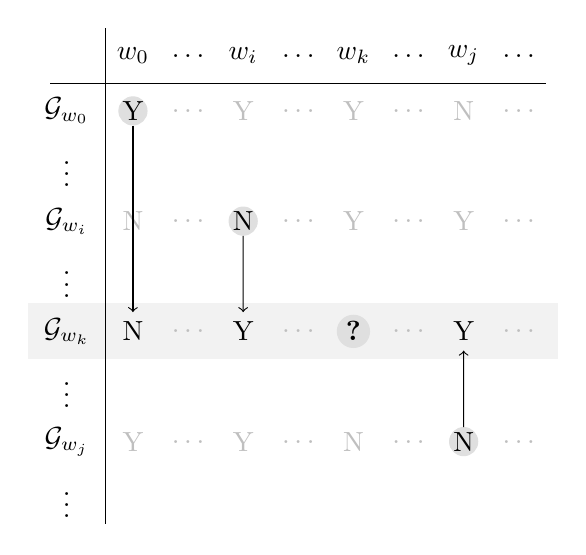
\begin{tikzpicture}[scale=0.7]

\draw[fill=lightgray!20, draw=lightgray!20] (-1.9,-3.5) rectangle (7.7,-4.5);

\node at (0,1) {$w_0$};
\node at (1,1) {$\dots$};
\node at (2,1) {$w_i$};
\node at (3,1) {$\dots$};
\node at (4,1) {$w_k$};
\node at (5,1) {$\dots$};
\node at (6,1) {$w_j$};
\node at (7,1) {$\dots$};

\node at (-1.2,0) {$\mathcal{G}_{w_0}$};
\node at (-1.2,-1) {$\vdots$};
\node at (-1.2,-2) {$\mathcal{G}_{w_i}$};
\node at (-1.2,-3) {$\vdots$};
\node at (-1.2,-4) {$\mathcal{G}_{w_k}$};
\node at (-1.2,-5) {$\vdots$};
\node at (-1.2,-6) {$\mathcal{G}_{w_j}$};
\node at (-1.2,-7) {$\vdots$};

\draw (-1.5, 0.5) to (7.5,0.5);
\draw (-0.5, 1.5) to (-0.5,-7.5);

\node[circle, draw=lightgray!50, fill=lightgray!50, inner sep=0] (00) at (0,0) {Y};
\node[lightgray] at (1,0) {$\ldots$};
\node[lightgray] at (2,0) {Y};
\node[lightgray] at (3,0) {$\ldots$};
\node[lightgray] at (4,0) {Y};
\node[lightgray] at (5,0) {$\ldots$};
\node[lightgray] at (6,0) {N};
\node[lightgray] at (7,0) {$\ldots$};

\node[lightgray] at (0,-2) {N};
\node[lightgray] at (1,-2) {$\ldots$};
\node[circle, draw=lightgray!50, fill=lightgray!50, inner sep=0] (ii) at (2,-2) {N};
\node[lightgray] at (3,-2) {$\ldots$};
\node[lightgray] at (4,-2) {Y};
\node[lightgray] at (5,-2) {$\ldots$};
\node[lightgray] at (6,-2) {Y};
\node[lightgray] at (7,-2) {$\ldots$};

\node (k0) at (0,-4) {N};
\node[lightgray] at (1,-4) {$\ldots$};
\node (ki) at (2,-4) {Y};
\node[lightgray] at (3,-4) {$\ldots$};
\node[circle, draw=lightgray!50, fill=lightgray!50, inner sep=1] (kk) at (4,-4) {\textbf{?}};
\node[lightgray] at (5,-4) {$\ldots$};
\node (kj) at (6,-4) {Y};
\node[lightgray] at (7,-4) {$\ldots$};

\node[lightgray] at (0,-6) {Y};
\node[lightgray] at (1,-6) {$\ldots$};
\node[lightgray] at (2,-6) {Y};
\node[lightgray] at (3,-6) {$\ldots$};
\node[lightgray] at (4,-6) {N};
\node[lightgray] at (5,-6) {$\ldots$};
\node[circle, draw=lightgray!50, fill=lightgray!50, inner sep=0] (jj) at (6,-6) {N};
\node[lightgray] at (7,-6) {$\ldots$};

\draw[->] (00) to (k0);
\draw[->] (ii) to (ki);
\draw[->] (jj) to (kj);

\end{tikzpicture}
	\caption{Illustration des Diagonalarguments beim Beweis, dass nicht jede entscheidbare Sprache \ch{1} ist}
\end{figure}






% \begin{Bemerkung}\
% 	\newcommand{\underarrowset}[2]{%
% 		\underset{%
% 			\mathclap{%
% 				\overset{\displaystyle\uparrow}{\mathclap{#1}}%
% 			}%
% 		}{#2}%
% 	}
% 	\begin{enumerate}
% 	\item Für "`$s(n)\leq n$"' betrachte 2-Band \ac{TM}, bei denen die Eingabe read-only ist und nur das zweite Arbeitsband der Platzschranke unterliegt (so ist $s(n)$ sublinear möglich).
% 	\item Jede Platzbeschränkung impliziert Laufzeitschranke.\\
% 	Angenommen Platzschranke $s(n)$\\
% 	$\curvearrowright$ \ac{TM} hat nur endlich viele Konfigurationen
% 	\[ N := \underarrowset{%
% 			\parbox{\widthof{\scriptsize Eingabeband}}{\raggedright\scriptsize Kopfpos. im Eingabeband}\hspace{1cm}
% 		}{n\vphantom{|}}
% 		|Q| \quad\cdot\quad
% 		\underarrowset{\parbox{2.2cm}{\scriptsize\centering mögliche Inhalte des Arbeitsbands}}{|\Gamma|}^{s(n)}
% 		\ \cdot\
% 		\underarrowset{\hspace{1.7cm}\parbox{2cm}{\scriptsize Kopfpos. auf\\ Arbeitsband}}{s(n)}
% 		\in 2^{O(\log n + s(n))}
% 	\]
% 	\item \ac{DTM} mit Platzschranke\,: $M$ entscheidet,\\
% 	falls sie akzeptiert, dann in weniger als $N$ Schritten,\\
% 	falls nach $N$ Schritten keine Terminierung erfolgt\\
% 	\quad$\curvearrowright$ Endlosschleife -- Abbruch
% 	\item \ac{NTM}\,: nutze den \ac{ND} optimistisch aus\,:\\
% 	falls eine akzeptierende Berechnung existiert, dann muss es eine Berechnung ohne wiederholte Konfiguration geben.
% 	\end{enumerate}
% \end{Bemerkung}
% \begin{Satz}[name={[$L\in\DTAPE(n),\ L\in\NTAPE(n)$]}]\label{satz:6.2}\
% 	\begin{itemize}
% 	\item $L\in\DTAPE(n) \curvearrowright\ \exists$ \ac{DTM}, die $L$ in Zeit $2^{O(n)}$ entscheidet.
% 	\item $L\in\NTAPE(n)$ analog.
% 	\end{itemize}
% \end{Satz}\vspace{-2em}
% \begin{proof}
% 	siehe oben.
% \end{proof}
% \begin{Bemerkung}
% 	Die Klasse $\NTAPE (n)$ heißt auch \ac{LBA}.
% \end{Bemerkung}
%


\begin{Satz}
	Die Typ-1-Sprachen sind abgeschlossen unter {\thinmuskip=6mu$\cup,\cap,\cdot,{}^*$} und Komplement.
\end{Satz}
\begin{proof}~
    \begin{itemize}
     \item "`$\cup$"' und "`$\cap$"':
     Betrachte eine \ac{NTM}.
     Seien $L_1$ und $L_2$ zwei Typ-1-Sprachen und $\M_1$ und $\M_2$ zwei zugehörige \ac{NTM}s.
     \begin{itemize}
     
     \item Verwende als Bandalphabet 2-Tupel, um eine 2-Spur-\ac{TM} zu simulieren.
     \item Verwende die untere Spur für eine "`Sicherungskopie"' der Eingabe.
     \item Simuliere auf der oberen Spur $\M_1$ und speichere das Ergebnis im Zustand.
     \item Simuliere auf der unteren Spur $\M_2$ und werte das Gesamtergebnis aus.
     \end{itemize}
     \item  "`$\cdot$"' und "`$^*$"':
     
     Konstruiere eine Typ-1-Grammatik analog zu \autoref{thm:cfl-closed-reg-intersect}.
     
     \item Komplement:
     
     "`2. \acsu{LBA}-Problem\footnote{\acs*{LBA} = \acl*{LBA} -- 1964 Kuroda}"' bis 1987, dann gelöst durch Immerman und Szelepcsényi.
     \qedhere
    \end{itemize}
\end{proof}
\begin{Bemerkung}
  "`1. \ac{LBA}-Problem (1964)"': Ist $\mathrm{NTAPE}(n) = \mathrm{DTAPE}(n)$? Bisher ungelöst.
\end{Bemerkung}

% \begin{Satz}
% 	Das Wortproblem für Typ-1-Sprachen ist entscheidbar.
% \end{Satz}
% \begin{proof}
% 	\begin{align*}
% 		L\in\mathcal{L}_1 &\curvearrowleftright L\in\mathrm{NTAPE}(n)\\
% 		&\curvearrowright \text{nach \autoref{satz:6.2}: $L$ entscheidbar}
% 	\end{align*}
% 	Nach \autoref{satz:6.1} sogar mit \ac{DTM}.
% \end{proof}
% Die Rückrichtung "`L entscheidbar. $\xcancel{\curvearrowright}\ L$ ist Typ-1-Sprache"' gilt nicht!

% \subsection{Typ-0 Sprachen}

\begin{Satz}\label{satz:6.6}
\ch{0} ist die Menge der semi-entscheidbaren Sprachen.
% 	$\mathcal{L}_0 = \ac{NTM}$
\end{Satz}
\begin{proof}
	\begin{itemize}
	\item["'\=>"'] Verwende die Konstruktion einer \ac{NTM} $\M$ wie in \autoref{satz:6.3}, aber ohne Platzbeschränkung.
	\item["'\<="'] Konstruktion analog zu \autoref{satz:6.3} + Startsymbol $S'$
	\begin{align*}
		S' &\-> \pmqty{\blank\\\Eps} S' \pmqty{\blank\\\Eps} &&\text{Schaffe Platz für Berechnung von }\M\\
		S' &\-> S\\
	\shortintertext{Erweitere $N$}
		&= \{S',S\}\cup\triangle\x(\Sigma\cup\{\Eps\})\\
	\shortintertext{Neue Löschregeln:}
		\pmqty{x\\ \Eps } &\-> \Eps &&\forall x\in\Gamma\\
		\rotatebox{90}{$\Rsh$}\ &\mathrlap{\text{die einzigen
                                          Regeln, die Typ-1-Bedingung verletzen.}} \tag*{\qedhere}
	\end{align*}
	\end{itemize}
\end{proof}

\begin{Satz}
 Die entscheidbaren Sprachen sind eine echte Teilmenge von $\ch{0}$.
\end{Satz}
\begin{proof}~
 \begin{itemize}
  \item "`$\subseteq$"':
  Folgt trivialerweise aus \autoref{def:semiEntscheidbar}, \autoref{def:tmAkzeptanz} und \autoref{def:entscheidbarkeit}.
  
  \item "`$\neq$"':
  Das spezielle Halteproblem ist nicht entscheidbar (\autoref{satz:speziellesHalteproblem}),
  aber semi-entscheidbar (\autoref{lemma:Ksemi-entscheidbar}).
  \qedhere
 \end{itemize}
\end{proof}




\begin{Satz}
 $\ch{0}\neq \calP(\Sigma^*)$
\end{Satz}
\begin{proof}
 Nach \autoref{kor:6.11} ist $\overline{K}$ nicht semi-entscheidbar.
\end{proof}



\begin{Satz}[name={[Abgeschlossenheit von Typ-0 Sprachen]}]\label{satz:Typ-0-abgeschl}
	Die Typ-0 Sprachen sind unter $\thinmuskip=6mu\cup,\cap,\cdot,{}^*$ abgeschlossen, sind aber nicht unter Komplementbildung abgeschlossen.
\end{Satz}
\begin{proof}~
    \begin{itemize}
     \item "`$\cup$"' und "`$\cap$"':
     
     Siehe \autoref{satz:SemidetCupCap}.

     \item  "`$\cdot$"' und "`$^*$"':
     
     Konstruiere Grammatik analog zu \autoref{thm:cfl-closed-reg-intersect}.
     
     \item Komplement:
     
     Das spezielle Halteproblem $K$ ist semi-entscheidbar (\autoref{lemma:Ksemi-entscheidbar}),
     aber sein Komplement $\overline{K}$ ist nicht semi-entscheidbar (\autoref{kor:6.11}).
     \qedhere
     \end{itemize}
\end{proof}

% \begin{Bem}
% 	Typ-0 Sprachen sind \emph{nicht} unter Komplement abgeschlossen!
% \end{Bem}
% 
% 
% \begin{Korollar}
% 	$\mathcal{L}_0 \supsetneqq \mathcal{L}_1$
% \end{Korollar}
% \begin{proof}
% 	$K$ ist unentscheidbar (also $\notin \mathcal{L}_1$), aber semi-entscheidbar (also $\in \mathcal{L}_0$).
% \end{proof}
}
